\begin{figure}[htbp]
\centering
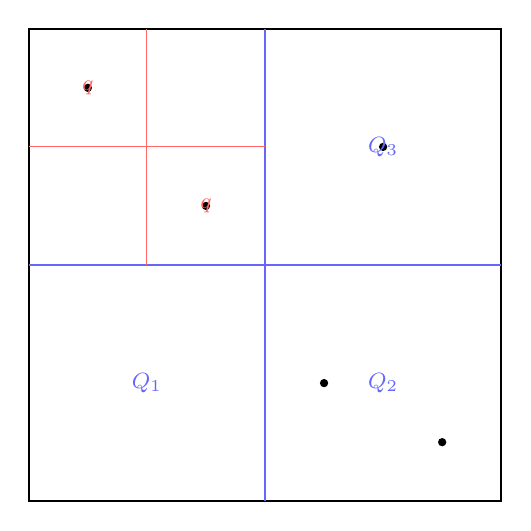
\begin{tikzpicture}[scale=0.75]
  \draw[thick] (0,0) rectangle (8,8);
  \draw[blue!60] (4,0)--(4,8);
  \draw[blue!60] (0,4)--(8,4);
  \draw[red!60] (2,4)--(2,8);
  \draw[red!60] (0,6)--(4,6);
  \fill (1,7) circle (2pt);
  \fill (3,5) circle (2pt);
  \fill (6,6) circle (2pt);
  \fill (5,2) circle (2pt);
  \fill (7,1) circle (2pt);
  \node[font=\footnotesize,blue!60] at (2,2) {$Q_1$};
  \node[font=\footnotesize,blue!60] at (6,2) {$Q_2$};
  \node[font=\footnotesize,blue!60] at (6,6) {$Q_3$};
  \node[font=\footnotesize,red!60] at (1,7) {$q$};
  \node[font=\footnotesize,red!60] at (3,5) {$q$};
\end{tikzpicture}
\caption{Quadtree: recursive 2D space partitioning. Quadrants with multiple points are subdivided; leaf quadrants contain at most one point.}
\label{fig:quadtree}
\end{figure}
